\documentclass[11pt,a4paper]{article}

\usepackage[margin=2.2cm]{geometry}
\usepackage{amsmath,amssymb,bm}
\usepackage{graphicx}
\usepackage{subcaption}
\usepackage{booktabs}
\usepackage{array}
\usepackage{multirow}
\usepackage{tabularx}
\usepackage{float}
\usepackage{xcolor}
\usepackage{listings}
\usepackage{enumitem}
\usepackage{xurl}
\usepackage{hyperref}
\usepackage{fancyhdr}
\usepackage{CJKutf8}

\graphicspath{{imgs/}}
\setlength{\parindent}{2em}
\setlength{\parskip}{0.35em}
\setlist{nosep}

\definecolor{linkblue}{HTML}{1756A9}
\definecolor{codegreen}{HTML}{26734D}
\definecolor{codegray}{HTML}{666666}
\definecolor{codebg}{HTML}{F5F7FA}
\hypersetup{
  colorlinks=true,
  linkcolor=linkblue,
  citecolor=linkblue,
  urlcolor=linkblue,
  pdftitle={Lab2 - DDIM and LoRA},
  pdfauthor={請填入姓名}
}

\lstdefinestyle{pythonstyle}{
  language=Python,
  basicstyle=\ttfamily\small,
  keywordstyle=\color{linkblue}\bfseries,
  commentstyle=\color{codegreen},
  stringstyle=\color{orange!70!black},
  numbers=left,
  numberstyle=\scriptsize\color{codegray},
  stepnumber=1,
  numbersep=8pt,
  frame=single,
  rulecolor=\color{black!15},
  backgroundcolor=\color{codebg},
  showstringspaces=false,
  columns=fullflexible,
  keepspaces=true,
  breaklines=true,
  tabsize=4
}
\lstset{style=pythonstyle}

% \pagestyle{fancy}
% \fancyhf{}
% \lhead{NYCU Image and Video Generation}
% \rhead{Lab2 - DDIM and LoRA}
% \cfoot{\thepage}
% \renewcommand{\headrulewidth}{0.4pt}

\author{應數所 \quad 王元亨 \quad 315652003}
\date{}

\newcommand{\reporttitle}[1]{
  \title{#1 \\[0.5em] Image and Video Generation}
  \maketitle
  % \begin{center}
  %   \large Image and Video Generation - Assignment 1
  % \end{center}
  % \vspace{0.5em}
}

\newcommand{\placeholder}[1]{\textcolor{red!75!black}{\textbf{#1}}}
\newcommand{\code}[1]{\texttt{#1}}

\begin{document}
\begin{CJK*}{UTF8}{bkai}
% \begin{titlepage}
%   \centering
%   \vspace*{2.2cm}
%   {\Large National Yang Ming Chiao Tung University\par}
%   \vspace{0.5cm}
%   {\Large Image and Video Generation\par}
%   \vspace{1.8cm}
%   {\Huge\bfseries Lab2\par}
%   \vspace{0.35cm}
%   {\LARGE\bfseries DDIM and LoRA\par}
%   \vfill
%   \begin{tabular}{rl}
%     姓名： & 王元亨 \\
%     學號： & 315652003 \\
%     日期： & \today
%   \end{tabular}
%   \vfill
% \end{titlepage}

\reporttitle{\textbf{Lab 2 - DDIM and LoRA}}
\vspace{1em}
\begin{abstract}
本實驗包含兩個主題。第一部分實作 Denoising Diffusion Implicit Models（DDIM），先在二維 Swiss Roll 資料上驗證反向生成流程，再將相同概念套用至預訓練影像擴散模型，分析推論步數與隨機性參數 $\eta$ 對 Fr\'echet Inception Distance（FID）的影響。第二部分使用 Low-Rank Adaptation（LoRA）微調 Stable Diffusion，分別學習 Naruto 視覺風格，以及透過 DreamBooth with LoRA 學習特定貓咪的身份。
\end{abstract}
\vspace{1.5em}
\tableofcontents
\clearpage

\section{Task 1：Denoising Diffusion Implicit Models}

\subsection{Task 1-1：2D Swiss Roll}

\subsubsection{實驗目的與前置 DDPM 元件}

令 $x_0$ 為真實資料、$\epsilon\sim\mathcal{N}(0,I)$，DDPM 的前向加噪可直接寫為
\begin{equation}
  x_t=\sqrt{\bar{\alpha}_t}x_0+\sqrt{1-\bar{\alpha}_t}\epsilon,
  \qquad
  \bar{\alpha}_t=\prod_{s=1}^{t}\alpha_s.
\end{equation}
程式中的 \code{q\_sample} 依此公式產生 $x_t$；\code{compute\_loss} 隨機抽取 timestep，讓網路預測加入的噪聲，並以
\begin{equation}
  \mathcal{L}_{\mathrm{simple}}
  =\mathbb{E}_{x_0,t,\epsilon}
  \left[\left\|\epsilon-\epsilon_\theta(x_t,t)\right\|_2^2\right]
\end{equation}
作為訓練目標。二維噪聲預測器由多層 \code{TimeLinear} 組成，將 sinusoidal timestep embedding 轉換後乘入各層特徵；最後一層投影回二維噪聲。\code{p\_sample} 實作單步 DDPM posterior sampling，\code{p\_sample\_loop} 則從高斯噪聲開始逐步走完所有訓練 timesteps。這些元件提供可用的噪聲預測網路，之後只更換反向取樣規則為 DDIM。

\subsubsection{DDIM 單步反向取樣}

在當前 timestep $t$，由網路得到 $\epsilon_\theta(x_t,t)$，首先估計乾淨資料：
\begin{equation}
  \hat{x}_0=
  \frac{x_t-\sqrt{1-\bar{\alpha}_t}\,\epsilon_\theta(x_t,t)}
       {\sqrt{\bar{\alpha}_t}}.
\end{equation}
接著以 $\eta$ 控制每一步的隨機程度：
\begin{equation}
  \sigma_t=\eta
  \sqrt{\frac{1-\bar{\alpha}_{t'}}{1-\bar{\alpha}_t}}
  \sqrt{1-\frac{\bar{\alpha}_t}{\bar{\alpha}_{t'}}},
\end{equation}
其中 $t'$ 是下一個較小的 inference timestep。更新式為
\begin{equation}
  x_{t'}=
  \sqrt{\bar{\alpha}_{t'}}\hat{x}_0
  +\sqrt{1-\bar{\alpha}_{t'}-\sigma_t^2}\,epsilon_\theta(x_t,t)
  +\sigma_t z,
  \qquad z\sim\mathcal{N}(0,I).
\end{equation}
當 $\eta=0$ 時，$\sigma_t=0$，在固定初始噪聲的條件下更新為 deterministic DDIM。

\begin{lstlisting}[caption={\code{ddim\_p\_sample}}]
alpha_t = extract(self.var_scheduler.alphas_cumprod, t, xt)
alpha_prev = (
    extract(self.var_scheduler.alphas_cumprod, t_prev, xt)
    if t_prev >= 0 else torch.ones_like(alpha_t)
)
eps_theta = self.network(xt, t)
x0_pred = (xt - torch.sqrt(1 - alpha_t) * eps_theta) / torch.sqrt(alpha_t)

sigma_t = eta * torch.sqrt((1 - alpha_prev) / (1 - alpha_t)) \
              * torch.sqrt(1 - alpha_t / alpha_prev)
direction = torch.sqrt(1 - alpha_prev - sigma_t ** 2) * eps_theta
noise = torch.randn_like(xt) if eta > 0 else torch.zeros_like(xt)
x_prev = torch.sqrt(alpha_prev) * x0_pred + direction + sigma_t * noise
\end{lstlisting}

\subsubsection{DDIM inference loop}

\code{ddim\_p\_sample\_loop} 先由訓練步數與指定推論步數計算
\begin{equation}
  r=\left\lfloor\frac{T_{\mathrm{train}}}{T_{\mathrm{infer}}}\right\rfloor,
\end{equation}
再建立由大到小排列的 timestep 子集合。取樣從標準高斯噪聲開始，每次呼叫單步 DDIM 更新，直到 $t'<0$ 時令 $\bar{\alpha}_{t'}=1$，得到最終 $x_0$。

\begin{lstlisting}[caption={\code{ddim\_p\_sample\_loop} timestep }]
step_ratio = self.var_scheduler.num_train_timesteps // num_inference_timesteps
timesteps = (
    (np.arange(num_inference_timesteps) * step_ratio)
    .round()[::-1].copy().astype(np.int64)
)
prev_timesteps = timesteps - step_ratio

xt = torch.randn(shape).to(self.device)
for t, t_prev in zip(timesteps, prev_timesteps):
    xt = self.ddim_p_sample(xt, t, t_prev, eta=eta)
\end{lstlisting}

\subsubsection{Swiss Roll 評估結果}

圖~\ref{fig:swiss-roll} 顯示目標分布與 DDIM 生成樣本。多數生成點能沿著兩圈 Swiss Roll 排列，僅有少量點落在曲線之外。Chamfer Distance 為 $18.4572$。

\begin{figure}[H]
  \centering
  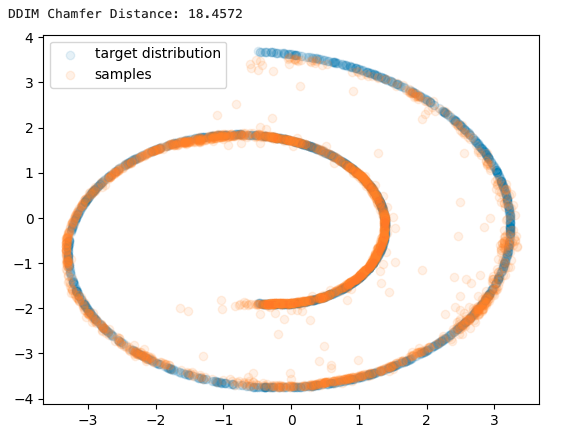
\includegraphics[width=0.72\textwidth]{task1-1-sample-cd.png}
  \caption{DDIM 在 Swiss Roll 上的生成結果與 Chamfer Distance。}
  \label{fig:swiss-roll}
\end{figure}

\subsection{Task 1-2：DDIM Image Generation}

\subsubsection{Inference timestep 設定}

影像實驗沿用 Lab 1 noise-prediction checkpoint 的 beta schedule，避免訓練與推論的 $\bar{\alpha}_t$ 不一致。\code{set\_inference\_timesteps} 依指定步數建立訓練 timestep 的子集合，並記錄相鄰 inference steps 的間距。

\begin{lstlisting}[caption={\code{DDIMScheduler.set\_inference\_timesteps}}]
step_ratio = self.num_train_timesteps // num_inference_timesteps
timesteps = (
    (np.arange(num_inference_timesteps) * step_ratio)
    .round()[::-1].copy().astype(np.int64)
)
self.timesteps = torch.from_numpy(timesteps)
self._ddim_step_ratio = step_ratio
\end{lstlisting}

\subsubsection{DDIMScheduler 單步更新}

先計算 $t'=t-r$，再由 $\epsilon_\theta$ 推回 $\hat{x}_0$；因影像已正規化至 $[-1,1]$，程式將 $\hat{x}_0$ clamp 至合法範圍以降低數值誤差。最後依前述 DDIM 方程式組合 predicted sample、direction term 與隨機項。$\eta=0$ 時不建立額外噪聲；$\eta>0$ 時則加入 $\sigma_tz$。

\begin{lstlisting}[caption={\code{DDIMScheduler.step}}]
t_prev = t - self._ddim_step_ratio
alpha_t = self._get_teeth(self.alphas_cumprod, t_tensor)
alpha_prev = (
    self._get_teeth(self.alphas_cumprod, t_prev_tensor)
    if t_prev >= 0 else torch.ones_like(alpha_t)
)
x0_pred = (x_t - torch.sqrt(1 - alpha_t) * eps_theta) / torch.sqrt(alpha_t)
x0_pred = x0_pred.clamp(-1.0, 1.0)

sigma_t = self.eta * torch.sqrt((1 - alpha_prev) / (1 - alpha_t)) \
                   * torch.sqrt(1 - alpha_t / alpha_prev)
direction = torch.sqrt(1 - alpha_prev - sigma_t ** 2) * eps_theta
noise = torch.randn_like(x_t) if self.eta > 0 else torch.zeros_like(x_t)
sample_prev = torch.sqrt(alpha_prev) * x0_pred + direction + sigma_t * noise
\end{lstlisting}

\subsubsection{實驗設定}

每一組設定生成 500 張影像，並以 AFHQ evaluation set 為 reference 計算 FID。除 DDIM inference steps 與 $\eta$ 外，其餘條件保持一致。

% \begin{table}[H]
%   \centering
%   \caption{Task 1-2 實驗設定。}
%   \begin{tabular}{ll}
%     \toprule
%     項目 & 設定 \\
%     \midrule
%     Predictor & noise \\
%     DDIM steps & 10, 20, 50, 100, 1000 \\
%     $\eta$ & 0.0, 0.2, 0.5, 1.0 \\
%     每組生成數量 & 500 \\
%     評估指標 & FID（越低越好） \\
%     Reference set & \code{data/afhq/eval} \\
%     \bottomrule
%   \end{tabular}
% \end{table}

\subsubsection{FID 結果與討論}

\begin{table}[H]
  \centering
  \caption{不同 DDIM steps 與 $\eta$ 的 FID。粗體為全體最佳結果。}
  \label{tab:fid}
  \begin{tabular}{c|rrrrr}
    \toprule
    \multirow{2}{*}{$\eta$} & \multicolumn{5}{c}{DDIM steps} \\
    \cmidrule(lr){2-6}
      & 10 & 20 & 50 & 100 & 1000 \\
    \midrule
    0.0 & 39.52 & 29.93 & 19.12 & 12.16 & 41.93 \\
    0.2 & 38.85 & 30.29 & 17.01 & 10.71 & 27.71 \\
    0.5 & 35.62 & 25.83 & 16.73 & 12.12 & \textbf{6.82} \\
    1.0 & 54.74 & 34.79 & 21.86 & 15.06 & 7.40 \\
    \bottomrule
  \end{tabular}
\end{table}
\newpage
由表~\ref{tab:fid} 可觀察到三點。第一，在 $\eta=0.5$ 與 $\eta=1.0$ 時，增加 inference steps 能穩定改善 FID；例如 $\eta=0.5$ 由 10 steps 的 $35.62$ 降至 1000 steps 的 $6.82$。第二，step 數很少時過大的隨機性會傷害品質，10 steps、$\eta=1.0$ 的 FID $54.74$ 為最差結果。第三，$\eta=0$ 與 $\eta=0.2$ 在 1000 steps 出現反常退化，顯示更多步數不必然保證較佳結果；可能原因包括 deterministic trajectory 對 checkpoint 誤差的累積、有限樣本造成的 FID 波動，或不同隨機起點造成的估計差異。若要驗證此現象，可固定 seed 並重複生成多組 500 張樣本，回報平均值與標準差。

圖~\ref{fig:fid-samples} 選擇最差與最佳設定的單張輸出作定性比較。低 FID 組合的紋理與輪廓較清楚，但單張影像僅作視覺輔助，主要結論仍以 500 張樣本計算的 FID 為準。

\begin{figure}[H]
  \centering
  \begin{subfigure}[t]{0.4\textwidth}
    \centering
    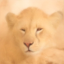
\includegraphics[width=\linewidth]{task1-2-sample-10-1.0.png}
    \caption{10 steps，$\eta=1.0$，FID 54.74。}
  \end{subfigure}
  \hspace{1.5em}
  \begin{subfigure}[t]{0.4\textwidth}
    \centering
    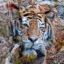
\includegraphics[width=\linewidth]{task1-2-sample-1000-0.5.png}
    \caption{1000 steps，$\eta=0.5$，FID 6.82。}
  \end{subfigure}
  \caption{不同 DDIM 設定的代表性生成影像。}
  \label{fig:fid-samples}
\end{figure}

\clearpage
\section{Task 2：Training Custom LoRA Models}

\subsection{方法簡介}

LoRA 將原始權重 $W$ 凍結，只訓練低秩更新：
\begin{equation}
  W'=W+\Delta W,\qquad \Delta W=BA,
\end{equation}
其中秩 $r$ 遠小於原權重維度，因此可用較少參數讓預訓練模型適應新風格或身份。本實驗以 Stable Diffusion v1.4 為 base model，分別訓練 style LoRA 與 DreamBooth LoRA。

\subsection{Task 2-1：Naruto Style LoRA}

\subsubsection{資料集與訓練設定}

本實驗使用 Hugging Face 上的 \href{https://huggingface.co/datasets/lambdalabs/naruto-blip-captions}{\code{lambdalabs/naruto-blip-captions}}。資料集由 Naruto 動畫影像及 BLIP 產生的文字描述組成，適合用來學習角色線條、色彩與動畫式陰影。圖~\ref{fig:naruto-data} 左側為資料範例，右側示範相同 prompt 在 LoRA 前後的外觀差異。

\begin{table}[H]
  \centering
  \caption{Style LoRA 訓練設定。}
  \begin{tabular}{ll}
    \toprule
    項目 & 設定 \\
    \midrule
    Base model & \code{CompVis/stable-diffusion-v1-4} \\
    Dataset & \code{lambdalabs/naruto-blip-captions} \\
    Resolution & $512\times512$ \\
    Batch size & 1 \\
    Epochs & 100 \\
    Learning rate & $1\times10^{-4}$ \\
    Scheduler & constant \\
    Seed & 42 \\
    \bottomrule
  \end{tabular}
\end{table}

\begin{figure}[H]
  \centering
  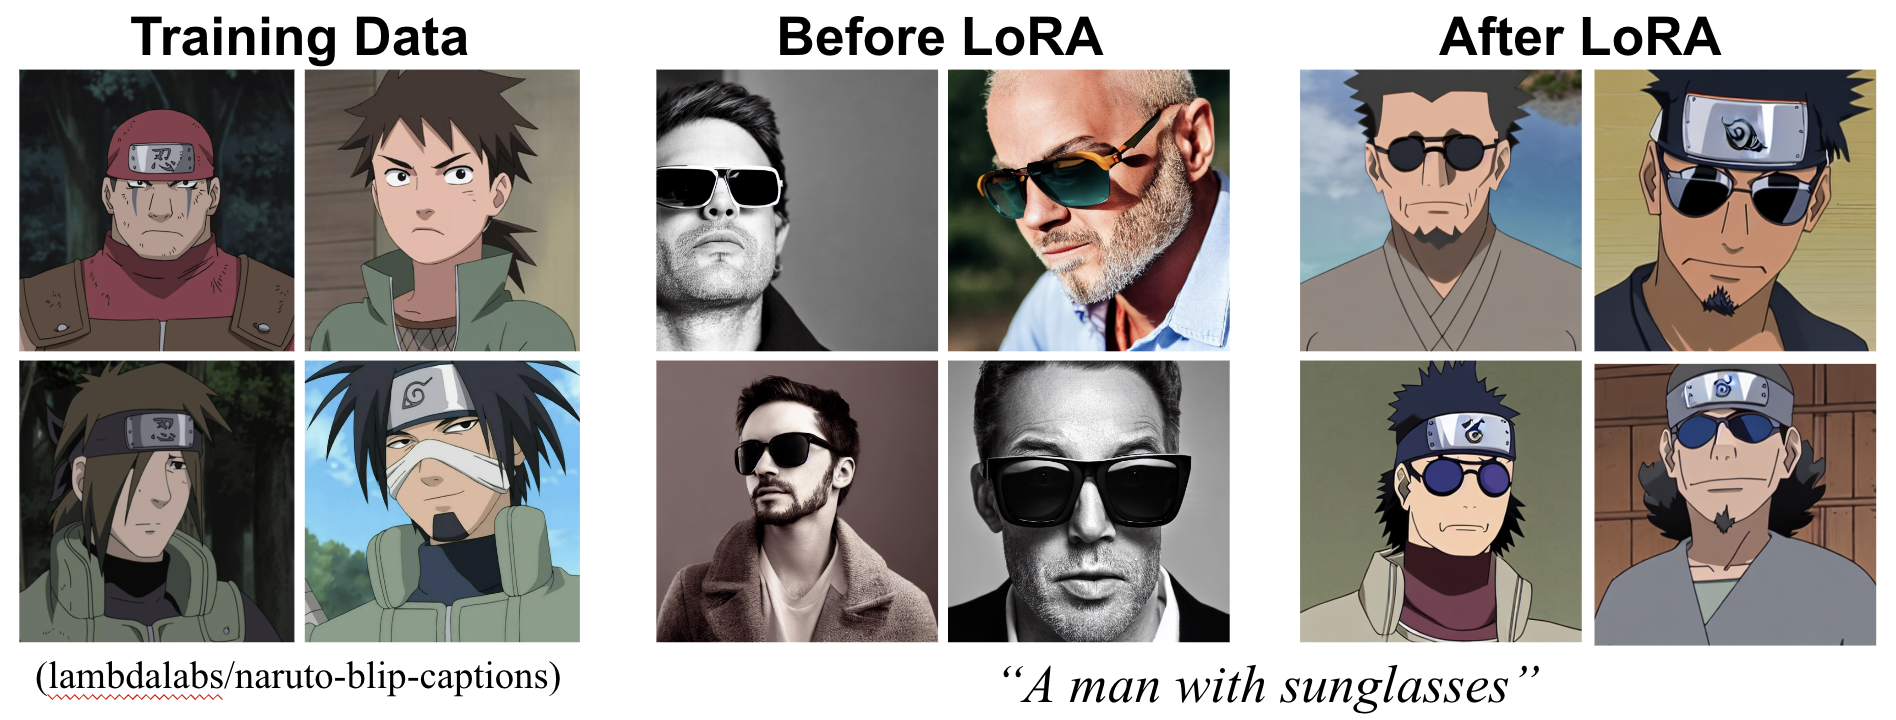
\includegraphics[width=\textwidth]{lora_example.png}
  \caption{Naruto LoRA 的代表性訓練資料，以及載入 LoRA 前後的生成差異。圖片來源為課程提供範例。}
  \label{fig:naruto-data}
\end{figure}

\subsubsection{生成結果}

為避免 prompt 本身直接指定動畫風格，以下 prompts 不包含 ``Naruto style'' 或 ``anime style''。結果顯示人物、動物與動作場景都呈現較一致的動畫線條、平面色彩與陰影，表示 LoRA 學到可轉移的視覺風格，而非只記住單一角色。

\begin{figure}[H]
  \centering
  \begin{subfigure}[t]{0.31\textwidth}
    \centering
    
\includegraphics[width=\linewidth]{naruto_man_sunglasses_seed100.png}
    \caption{\footnotesize\code{a man with sunglasses}}
  \end{subfigure}
  \hfill
  \begin{subfigure}[t]{0.31\textwidth}
    \centering
    
\includegraphics[width=\linewidth]{naruto_swordsman_action_pose_seed100.png}
    \caption{\footnotesize\code{a young swordsman fighting in a bamboo forest, dynamic action pose}}
  \end{subfigure}
  \hfill
  \begin{subfigure}[t]{0.31\textwidth}
    \centering
    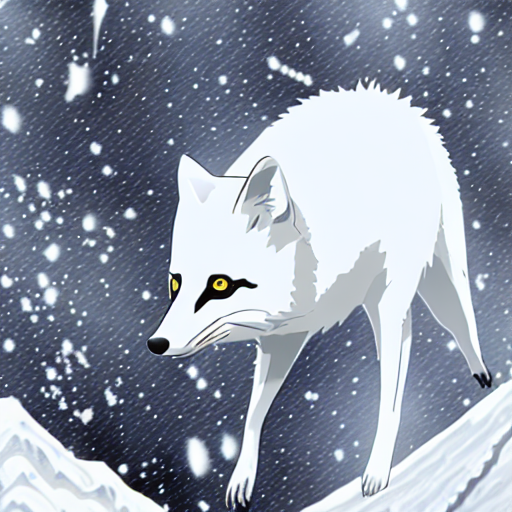
\includegraphics[width=\linewidth]{naruto_fox_running_seed100.png}
    \caption{\footnotesize\code{a white fox running across a snowy mountain}}
  \end{subfigure}
  \caption{Style LoRA 的生成結果}
  \label{fig:naruto-results}
\end{figure}

\paragraph{LoRA 權重}
Style LoRA 權重上傳於 \href{https://github.com/albertwang1104/Lab2-DDIM-LoRA/blob/main/task2/weights/naruto_lora.safetensors}{GitHub}。


\subsection{Task 2-2：DreamBooth with LoRA}

\subsubsection{資料集與訓練設定}

本實驗使用課程 repository 提供的四張橘色長毛貓影像，並以稀有識別詞 \code{sks cat} 綁定該身份。四張訓練圖具有不同視角、姿勢與室內背景，可幫助模型區分貓咪的固定外觀與可變場景。

\begin{figure}[H]
  \centering
  \begin{subfigure}[t]{0.23\textwidth}
    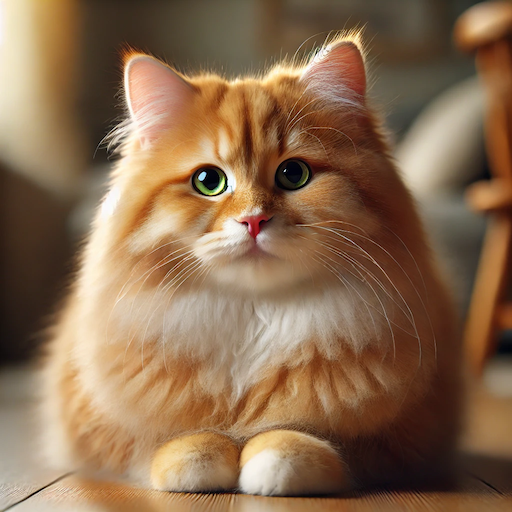
\includegraphics[width=\linewidth]{dreambooth_train_0.png}
  \end{subfigure}
  \hfill
  \begin{subfigure}[t]{0.23\textwidth}
    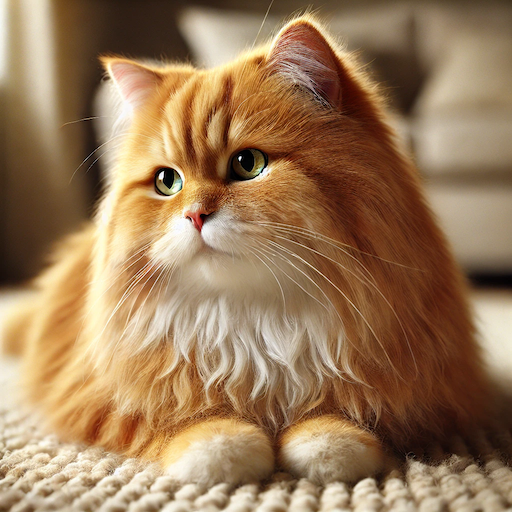
\includegraphics[width=\linewidth]{dreambooth_train_1.png}
  \end{subfigure}
  \hfill
  \begin{subfigure}[t]{0.23\textwidth}
    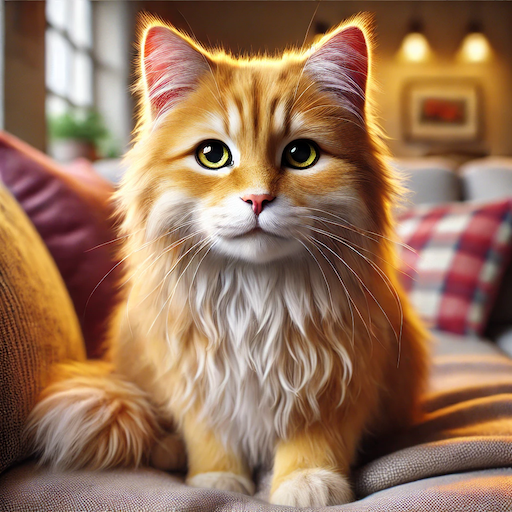
\includegraphics[width=\linewidth]{dreambooth_train_2.png}
  \end{subfigure}
  \hfill
  \begin{subfigure}[t]{0.23\textwidth}
    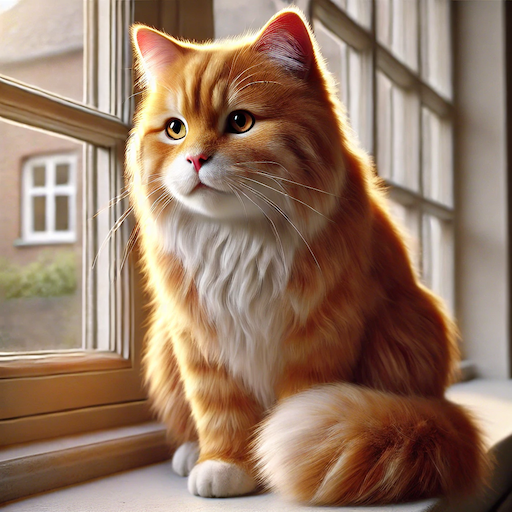
\includegraphics[width=\linewidth]{dreambooth_train_3.png}
  \end{subfigure}
  \caption{DreamBooth LoRA 使用的四張身份訓練影像。}
  \label{fig:dreambooth-data}
\end{figure}

\begin{table}[H]
  \centering
  \caption{DreamBooth LoRA 訓練設定。}
  \begin{tabular}{ll}
    \toprule
    項目 & 設定 \\
    \midrule
    Base model & \code{CompVis/stable-diffusion-v1-4} \\
    Instance prompt & \code{a photo of a sks cat} \\
    Resolution & $512\times512$ \\
    Batch size & 1 \\
    Maximum training steps & 500 \\
    Learning rate & $1\times10^{-4}$ \\
    Scheduler & constant \\
    Seed & 0 \\
    \bottomrule
  \end{tabular}
\end{table}

\subsubsection{生成結果}

前兩個推論 prompt 保留 \code{sks cat} 識別詞，並改變成訓練資料中沒有的海灘與桶子場景。圖~\ref{fig:dreambooth-results} 前兩張影像仍保留橘色長毛、白色胸毛及相近臉部特徵，顯示模型能在場景改變時維持主要身份特徵。第三張使用不含 \code{sks cat} 的 prompt \code{a man with sunglasses}，結果生成一般男性而非目標貓咪，可作為負向對照，說明身份識別詞是觸發 DreamBooth 個體概念的關鍵。另一方面，毛色飽和度與臉部細節仍會受 prompt、seed 與 base model prior 影響，因此身份重建並非像素級複製。

\begin{figure}[H]
  \centering
  \begin{subfigure}[t]{0.32\textwidth}
    \centering
    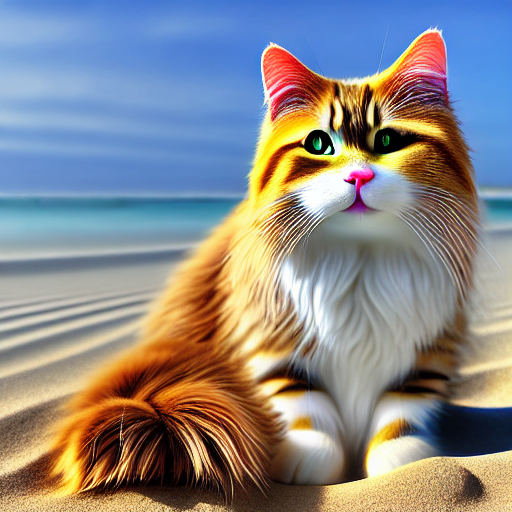
\includegraphics[width=\linewidth]{dreambooth_cat_beach_seed100.png}
    \caption{\code{a photo of sks cat on the beach}}
  \end{subfigure}
  \hfill
  \begin{subfigure}[t]{0.32\textwidth}
    \centering
    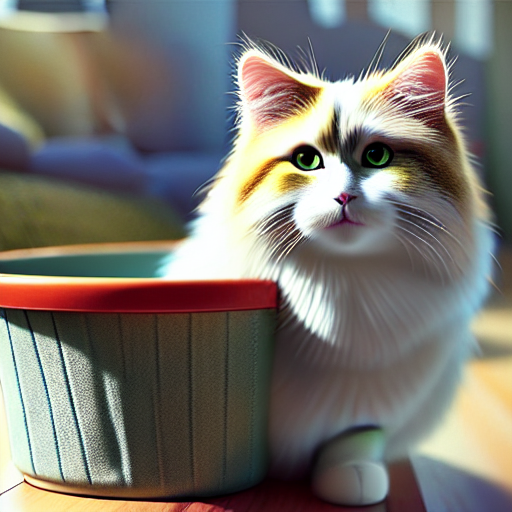
\includegraphics[width=\linewidth]{dreambooth_cat_bucket_seed100.png}
    \caption{\code{a photo of sks cat in a bucket}}
  \end{subfigure}
  \hfill
  \begin{subfigure}[t]{0.32\textwidth}
    \centering
    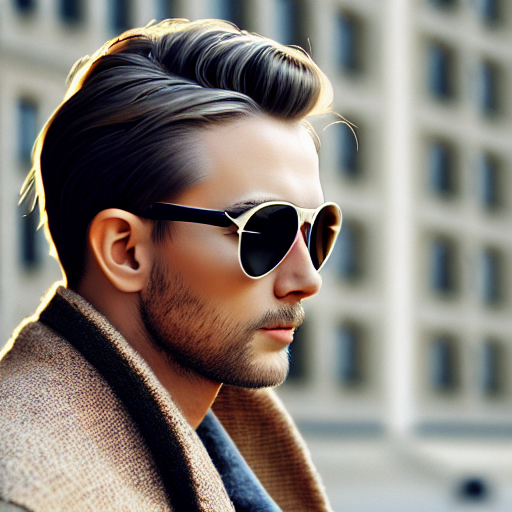
\includegraphics[width=\linewidth]{dreambooth_man_sunglasses_seed100.png}
    \caption{\code{a man with sunglasses}}
  \end{subfigure}
  \caption{DreamBooth LoRA 的生成結果}
  \label{fig:dreambooth-results}
\end{figure}

\paragraph{LoRA 權重}
DreamBooth LoRA 權重上傳於 \href{https://github.com/albertwang1104/Lab2-DDIM-LoRA/blob/main/task2/weights/dreambooth_cat_lora.safetensors}{GitHub}。


\section{結論}

本實驗完成二維與影像版本的 DDIM noise-prediction sampling。Swiss Roll 的 Chamfer Distance 為 $18.4572$；影像實驗的最佳組合為 1000 steps、$\eta=0.5$，FID 為 $6.82$。結果顯示減少反向步數可大幅加速生成，但步數過少時品質會下降；$\eta$ 的適當隨機性也會影響生成分布。LoRA 實驗則顯示，少量可訓練參數即可讓 Stable Diffusion 學習 Naruto 視覺風格；搭配 DreamBooth 與識別詞後，也能在不同場景中重現特定貓咪身份。

\begin{thebibliography}{9}

\bibitem{song2021ddim}
J. Song, C. Meng, and S. Ermon,
``Denoising Diffusion Implicit Models,''
\textit{International Conference on Learning Representations}, 2021.

\bibitem{ho2020ddpm}
J. Ho, A. Jain, and P. Abbeel,
``Denoising Diffusion Probabilistic Models,''
\textit{Advances in Neural Information Processing Systems}, 2020.

\bibitem{hu2022lora}
E. J. Hu et al.,
``LoRA: Low-Rank Adaptation of Large Language Models,''
\textit{International Conference on Learning Representations}, 2022.

\bibitem{ruiz2023dreambooth}
N. Ruiz et al.,
``DreamBooth: Fine Tuning Text-to-Image Diffusion Models for Subject-Driven Generation,''
\textit{IEEE/CVF Conference on Computer Vision and Pattern Recognition}, 2023.

\bibitem{naruto-dataset}
Lambda Labs,
``Naruto BLIP Captions,'' Hugging Face Datasets.\newline
\url{https://huggingface.co/datasets/lambdalabs/naruto-blip-captions}

\end{thebibliography}

\end{CJK*}
\end{document}
